%!TEX program = lualatex
\documentclass[xcolor={dvipsnames}]{beamer}
\usepackage[T1]{fontenc}
\usepackage[english]{babel}
\usepackage{amssymb}
\usepackage{amsmath}
\usepackage{tikz}
\usepackage{xcolor}
\usepackage{colortbl}
\usepackage{listings}
\usepackage{graphicx}
\renewcommand*\footnoterule{}
\graphicspath{ {./figures/} }


\date{tba}
\author{Til Roth}
\title{Can I Opt Out Yet? \\GDPR and the Global Illusion of Cookie Control}
\setbeamertemplate{footline}[page number]
\usetheme{metropolis}
\institute{Hot Topics in Data Networks WS22/23\\Saarland Informatics Campus}

\begin{document}
\maketitle

\section{Motivation}

\begin{frame}{Cookie Consent Notices}
	\begin{itemize}
		\item should allow privacy control on websites
		\item present on many websites
		\item result of the \emph{General Data Protection Regulation} (GDPR) issued by the European Union in 2018
	\end{itemize}
\end{frame}

\begin{frame}{GDPR}
	\begin{itemize}
		\item regulate privacy online for EU citizens
		\item restrict tracking online
		\item privacy policies should be readable
	\end{itemize}
\end{frame}

\begin{frame}{Outline}
    \begin{itemize}
        \item Technical Background
        \item Methodology
        \item Analysis
    \end{itemize}
\end{frame}

\section{Technical Background}

\begin{frame}{Tracking}
    \centering
    Cookie tracking vs fingerprinting
\end{frame}

\begin{frame}{GDPR}
    \begin{itemize}
        \item cookies that can uniquely identify a user\\(except essential cookies e.g. shopping cart)
        \item data stored not longer than necessary
        \item consent must be explicit
        \item privacy policies transparent and accessible
    \end{itemize}
\end{frame}

\section{Methodology}

\begin{frame}{Setup}
	\begin{itemize}
		\item Alexa top-1M websites
		\item 2000 websites of the top categories determined by Symantec RuleSpace
	\end{itemize}
\end{frame}

\begin{frame}{Data Collection}
    \begin{itemize}
        \item manual analysis
        \item always opt-out if possible
        \item different types of cookie notices:
            \begin{itemize}
                \item \emph{Anyway}
                \item \emph{AutoAccept}
                \item \emph{OnlyAccept}
                \item \emph{AcceptReject}
                \item \emph{JustSettings}
            \end{itemize}
    \end{itemize}
\end{frame}

\begin{frame}{Identifying Tracking Cookies}
    Common approach:
    \begin{itemize}
        \item known third-party tracker list
        \item probe cookie against list
    \end{itemize}

    \pause
    \vspace{2em}

    Approach of the underlying work:
    \begin{itemize}
        \item with xzcvbn
        \item entropy of the cookie value
    \end{itemize}
\end{frame}

\begin{frame}{Privacy Policies}
    \begin{itemize}
        \item copy HTML of the privacy policy
        \item FRES
        \item FKRL
    \end{itemize}
\end{frame}

\section{Analysis}

\begin{frame}{Type of Tracking}
    \centering
    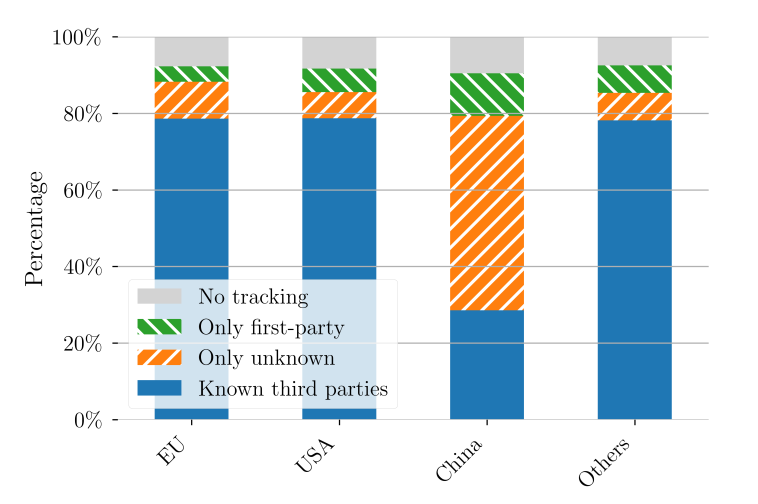
\includegraphics[scale=0.36]{figures/tracking_kind_trans.png}
\end{frame}

\begin{frame}{Size of Consent Notice}
    \centering
    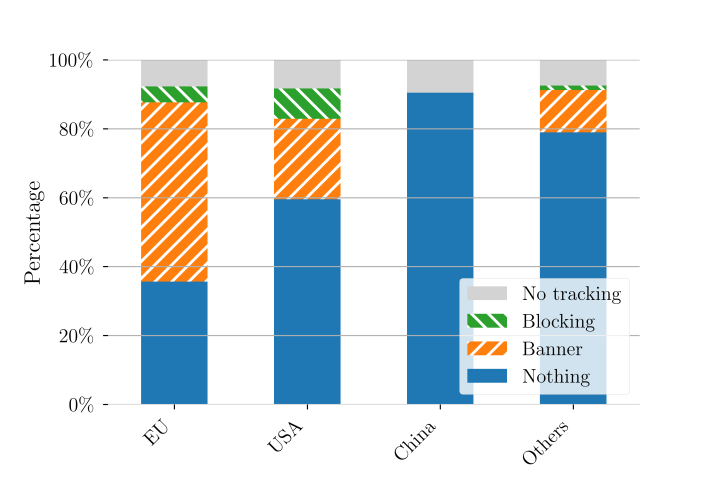
\includegraphics[scale=0.4]{figures/cookie_notice_size_trans.png}
\end{frame}

\begin{frame}{Type of Consent Notice}
    \centering
    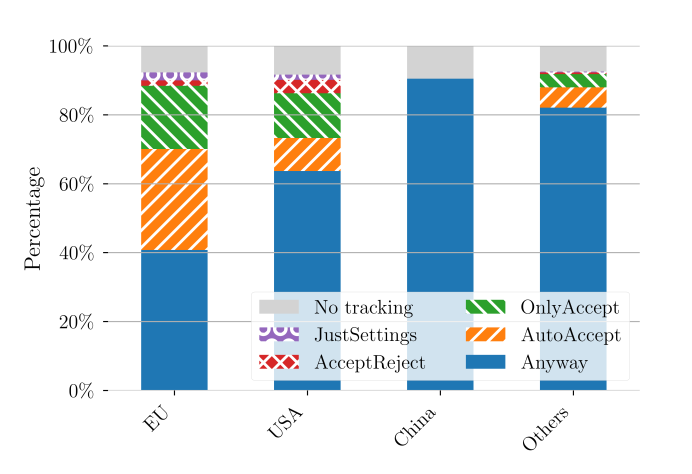
\includegraphics[scale=0.4]{figures/cookie_notice_type_trans.png}
\end{frame}

\begin{frame}{Third-Party opt-out}
    \centering
    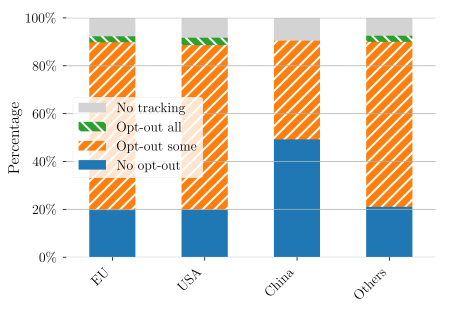
\includegraphics[scale=0.58]{figures/third_party_trans.png}
\end{frame}

\begin{frame}{Privacy Policies}
    Underlying work of 2019:\\
    \vspace{.5em}
    \centering
    \begin{tabular}{ l r r r }
        \hline
        Region & Policies & FRES & FKRL \\
        \hline
        EU & 190 & 57.1 & 10.5 \\
        USA & 617 & 54.5 & 11.2 \\
        All & 849 & 54.1 & 11.1 \\
        \hline
    \end{tabular}

    \vspace{1em}

    \begin{tabular}{ l r r }
        \hline
        & FRES & FKRL \\
        \hline
        2004 & 34.2 & 14.2 \\
        2019 & 54.1 & 11.1 \\
        goal & 65.0 & 8.0 \\
        \hline
    \end{tabular}
\end{frame}

% \begin{frame}{Limitations}
%
% \end{frame}

\begin{frame}{Conclusion}
    \begin{itemize}
        \item manual analysis of international websites
        \item GDPR had a global impact
        \item more information on privacy
        \item better readability of privacy policies
        \item tracking still ubiquitous
        \item cookie consent notices do not respect choice
    \end{itemize}
    \pause
    \centering
    \LARGE
    Thank you for your attention.
\end{frame}

\end{document}

